\documentclass[a4paper, 10.5pt]{article}

% IMPORTANT: Compile this file with XeLaTeX for proper font rendering.

% --- Preamble ---
\usepackage[left=1.0cm, right=1.0cm, top=1.4cm, bottom=1.4cm]{geometry}
\usepackage{graphicx}
\usepackage{xcolor}
\usepackage{fontspec}
\usepackage{enumitem}
\usepackage[explicit]{titlesec}
\usepackage{microtype}
\usepackage{fontawesome5}
\usepackage{hyperref}
\usepackage{etoolbox}
\usepackage{array}
\usepackage{tikz}
\newsavebox{\headerbox}

% --- Colors ---
\definecolor{PrimaryColor}{HTML}{003366}
\definecolor{DescriptionGray}{HTML}{444444}

% --- Fonts (XeLaTeX) ---
% Font source: project root fonts/ (site-wide font set).
% This file lives at static/uploads/CV_en.tex; relative path is ../../fonts/.

% Serif: CMU Serif
\setmainfont[
  Path = ../../fonts/cmu-serif/ ,
  Extension = .ttf,
  UprightFont = cmunrm,
  BoldFont = cmunbx,
  ItalicFont = cmunti,
  BoldItalicFont = cmunbi
]{CMU Serif}

% Sans Serif: CMU Sans Serif
\setsansfont[
  Path = ../../fonts/cmu-sans-serif/ ,
  Extension = .ttf,
  UprightFont = cmunss,
  BoldFont = cmunsx,
  ItalicFont = cmunsi,
  BoldItalicFont = cmunso
]{CMU Sans Serif}

% --- Hyperlinks ---
\hypersetup{
  colorlinks=true,
  linkcolor=PrimaryColor,
  urlcolor=PrimaryColor,
  citecolor=PrimaryColor,
  pdfborder={0 0 0},
}

% --- Global ---
\pagestyle{empty}
\setlength{\parindent}{0pt}
\setlength{\parskip}{0.4em}
\setlength{\emergencystretch}{3em}
\setlist{itemsep=0.2em, parsep=0pt, topsep=0.3em, leftmargin=1.2em}

% --- Section style ---
\titleformat{\section}
  {\normalfont\large\bfseries\color{PrimaryColor}}
  {}
  {0em}
  {#1}
  [\vspace{0.2ex}\hrule height 0.6pt]
\titlespacing*{\section}{0pt}{0.6ex}{1.0ex}

% --- Custom commands ---

% Subsection: primary-color bold small; flush with surrounding entries
\newcommand{\subSection}[1]{%
  \vspace{-0.15em}%
  \noindent{\color{PrimaryColor}\textbf{\small #1}}\par%
  \vspace{-0.1em}%
}

% Job entry: #1=Title@Org, #2=Date (optional), #3=Description (optional)
% Title flush-left, date pushed right via \hfill; description sits below title.
\newcommand{\jobEntry}[3]{%
  \noindent\textbf{#1}%
  \notblank{#2}{\hfill{\color{DescriptionGray}\small #2}}{}%
  \notblank{#3}{\par\vspace{0.05em}\noindent{\color{DescriptionGray}\small\textit{#3}}}{}%
  \par\vspace{0.45em}%
}

% Five-dot skill bar
\newcommand{\filledDot}{\textcolor{PrimaryColor}{\small\textbullet}}
\newcommand{\emptyDot}{\textcolor{DescriptionGray}{\small$\circ$}}
\newcommand{\skillRow}[2]{%
  % #1 = skill name, #2 = level 1-5
  #1 &
  \ifnum#2>0\filledDot\else\emptyDot\fi\,%
  \ifnum#2>1\filledDot\else\emptyDot\fi\,%
  \ifnum#2>2\filledDot\else\emptyDot\fi\,%
  \ifnum#2>3\filledDot\else\emptyDot\fi\,%
  \ifnum#2>4\filledDot\else\emptyDot\fi%
  \\
}

\begin{document}

% =====================================================================
% Header: photo overlaid in top-right via tikz; text centered on the page.
% =====================================================================
\sbox{\headerbox}{%
  \begin{minipage}{\dimexpr\textwidth-1cm\relax}
    \centering
    {\fontsize{22pt}{26pt}\selectfont\bfseries\color{PrimaryColor}Sichen Wang}\\[0.45em]
    {\color{DescriptionGray}
      \faIcon{graduation-cap}\ ECE · Sophomore \quad
      \faIcon{award}\ First-Class Scholarship \\[0.3em]
      \faIcon{phone}\ +86 19118814609 \quad
      \faIcon{envelope}\ \href{mailto:sichenwang@cuhk.edu.cn}{sichenwang@cuhk.edu.cn} \\[0.3em]
      \faIcon{github}\ \href{https://github.com/sichen-wang}{sichen-wang} \quad
      \raisebox{-0.2em}{
\includegraphics[height=1em]{yourphoto.png}}\ \href{https://sichen-wang.github.io}{sichen-wang.github.io}}
  \end{minipage}%
}

% Reserve vertical space for the header so subsequent content starts below.
\noindent\rule{0pt}{\dimexpr\ht\headerbox+\dp\headerbox\relax}%

% Place text and photo via tikz overlay with bottom-aligned photo.
\begin{tikzpicture}[remember picture, overlay]
  \node[anchor=north, inner sep=0pt] at
    ([xshift=-0.5cm, yshift=-1.4cm]current page.north)
    {\usebox{\headerbox}};
  \node[anchor=south east, inner sep=0pt] at
    ([xshift=-1.7cm, yshift={\dimexpr -1.4cm-\ht\headerbox-\dp\headerbox\relax}]current page.north east)
    {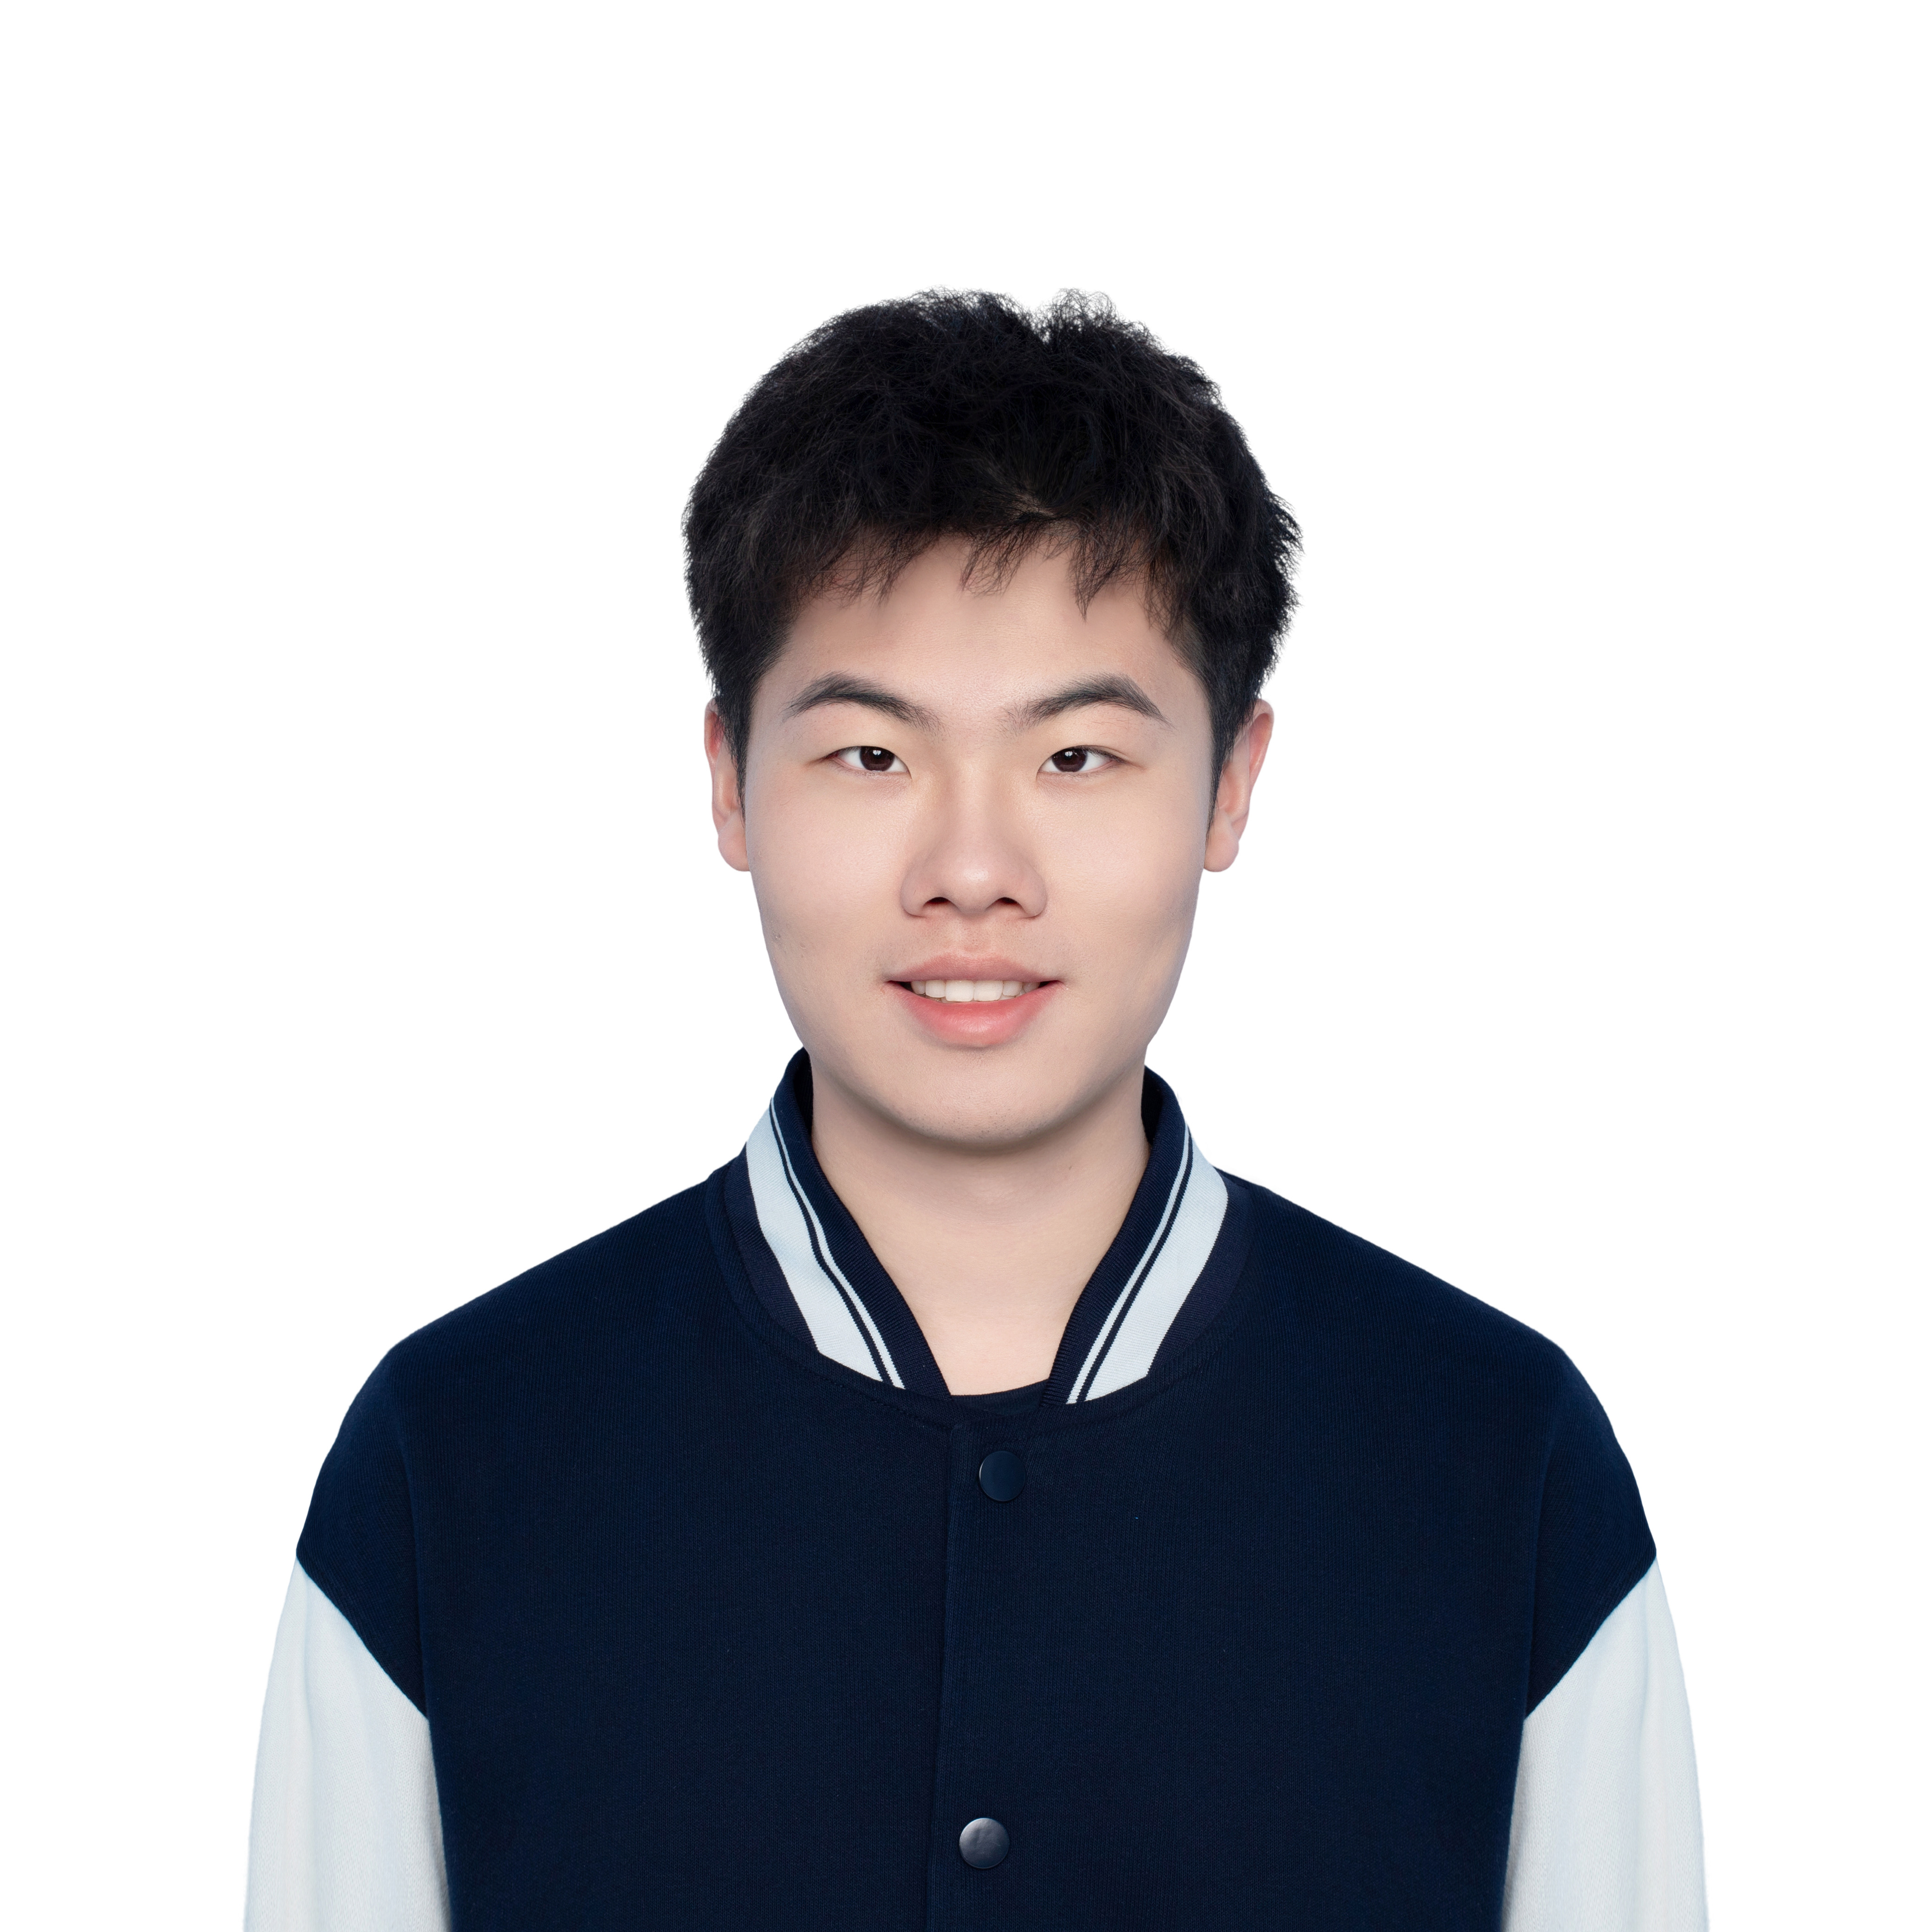
\includegraphics[height=\dimexpr\ht\headerbox+\dp\headerbox+0.5cm\relax, keepaspectratio]{photo.JPG}};
\end{tikzpicture}%

\vspace{-2.4em}

% =====================================================================
% Two-column body
% =====================================================================
\begingroup
\linespread{1.03}\selectfont
\begin{minipage}[t]{0.30\textwidth}
% 左栏偏窄：左对齐 + 禁连字断词，长项按词换行，避免两端对齐拉出大间隙
\raggedright\hyphenpenalty=10000\exhyphenpenalty=10000\relax

% --- Interests ---
\section{Interests}
{\color{DescriptionGray}
Theory of Algorithms\\[0.2em]
Learning Theory\\[0.2em]
Theoretical CS\\[0.2em]
Discrete Mathematics\\[0.2em]
Computational Mathematics
}

% --- Skills ---
\vspace*{-0.15em}
\section{Skills}
{\color{DescriptionGray}
\begin{tabular*}{\linewidth}{@{}l@{\extracolsep{\fill}}r@{}}
\skillRow{C++}{4}
\skillRow{Python}{4}
\skillRow{\LaTeX}{3}
\skillRow{MATLAB}{2}
\end{tabular*}}

% --- Languages ---
\vspace*{-0.15em}
\section{Languages}
{\color{DescriptionGray}
\begin{tabular*}{\linewidth}{@{}l@{\extracolsep{\fill}}r@{}}
Chinese & Native \\
English & B2 \\
Russian & A2 \\
\end{tabular*}}

% --- Hobbies ---
\vspace*{-0.15em}
\section{Hobbies}
{\color{DescriptionGray}
Piano / Violin\\[0.2em]
Drums (CMA Gr.\ 10, Distinction)\\[0.2em]
Badminton\\[-0.05em]
(Intramural Quarterfinalist)\\[0.2em]
50m Sprint 6.4s (Intramural 1st)\\[0.2em]
Debate\\[-0.05em]
(Intramural 2nd, Best Debater)
}

\end{minipage}%
\hfill
\begin{minipage}[t]{0.68\textwidth}

% --- Publications ---
\section{Publications}
\begingroup
\raggedright

\textbf{Sichen Wang}, Zhipeng Lu.\ \textit{Depth over Fidelity in Fixed-Budget Noisy Evolution Strategies}.\ Accepted at ICML 2026.

\textbf{Sichen Wang}, Zhipeng Lu.\ \textit{Preconditioned Implicit Midpoint Langevin Sampling for Non-Smooth Bayesian Imaging}.\ Submitted to NeurIPS 2026.

\textbf{Sichen Wang}.\ \textit{The Minimax Rate of Online Isotonic Regression on Product Orders}.\ Submitted to NeurIPS 2026.

Qihao Shi, Zeyu Wang, Jingbang Chen, \textbf{Sichen Wang}, Danni Ren, Wujian Yang, Guanlin Chen, Mingli Song, Can Wang.\ \textit{An Efficient Index Framework for Fast Query Processing on Dynamic Uncertain Graphs}.\ Submitted to IEEE Transactions on Knowledge and Data Engineering (TKDE).

Ruida Liu, Wang Xu, Shuoran Cheng, \textbf{Sichen Wang}, Weichao Pan, Han Puyu.\ \textit{DeepOcean-PT: Efficient Pressure-to-Temperature Profile Reconstruction for the Deep Ocean}.\ Submitted to IEEE Journal of Oceanic Engineering (JOE).

Jingbang Chen, \textbf{Sichen Wang}$^{\dagger}$.\ \textit{The Price of Order in the Logarithmic Method}.\ \mbox{Submitted to SODA 2027.}

\textbf{Sichen Wang}.\ \textit{The Movement Complexity of Sorting}.\ \mbox{Submitted to SODA 2027.}

\textbf{Sichen Wang}.\ \textit{The Complexity of Steering Rotor Walks}.\ \mbox{Submitted to SODA 2027.}

{\small\color{DescriptionGray}$^{\dagger}$ Theoretical computer science conference authors are listed alphabetically.}

\endgroup

% --- Awards ---
\section{Awards}
\begin{tabular*}{\linewidth}{@{}l @{\extracolsep{\fill}} >{\raggedleft\arraybackslash}p{2.8cm}@{\hspace{0.6em}} r@{}}
NOI 2022 Winter Camp & \textbf{Silver Medal} & \\
CSP-S / NOIp (3 consecutive years) & \textbf{First Prize} & \\
ICPC 2024 Asia Regional (Kunming, Shenyang) & \textbf{Gold Medal} & Top 3\% \\
CCPC 2024 China Collegiate Programming Contest & \textbf{Gold Medal} & Top 4\% \\
ICPC 2024 Asia East Continent Finals (EC-Final) & \textbf{Rank 31} & Top 11\% \\
CCF CSP Software Certification & \textbf{480/500 pts} & Top 0.1\% \\
AdventureX 2025 Hackathon & \textbf{Champion} & \\
\end{tabular*}

% --- Experience ---
\section{Experience}

\subSection{Research}
\jobEntry{Research Assistant @ CUHK-Shenzhen}{Dec.\ 2024 -- Present}{Frontier research on the foundations of large language models with Prof.\ Xiaoying Tang, School of Science and Engineering, The Chinese University of Hong Kong, Shenzhen.}
\jobEntry{Research Assistant @ SMBU}{Nov.\ 2025 -- Present}{Frontier research in computational mathematics with Prof.\ Zhipeng Lu, Faculty of Engineering, Shenzhen MSU-BIT University.}

\subSection{Industry}
\jobEntry{Algorithm Researcher @ RobustMotion}{May 2025 -- Present}{Authored an internal technical report; proposed the ``Turning-Potential Avoidance'' method for a class of data scheduling problems on planar grid graphs.}

\subSection{Competitive Programming}
\jobEntry{Lecturer @ NOI 2026 Hunan Provincial Team Training}{Apr.\ 2026}{}
\jobEntry{Lecturer @ Xuejun Xinyou Team Summer Camp}{Aug.\ 2026}{}
\jobEntry{Lecturer @ CCF Informatics Summer Camp}{Aug.\ 2023}{}
\jobEntry{Coach @ SMBU Experimental High School}{Aug.\ 2023 -- Feb.\ 2025}{Specially appointed by the principal as the informatics olympiad coach.}
\jobEntry{Problem Setter @ Nowcoder}{}{Solely responsible for problem setting and editorials of 6 contests, each with 2000+ participants.}

\end{minipage}
\endgroup

\end{document}
